%%% LaTeX Template: Article/Thesis/etc. with colored headings and special fonts
%%%
%%% Source: http://www.howtotex.com/
%%% Feel free to distribute this template, but please keep to referal to http://www.howtotex.com/ here.
%%% February 2011
%%%
%%% Modified October 2015 by CDM

%%%  Preamble
\documentclass[11pt,letterpaper]{article}
\usepackage[margin=1.0in]{geometry}
\usepackage[T1]{fontenc}
\usepackage[bitstream-charter]{mathdesign}
\usepackage[latin1]{inputenc}
\usepackage{amsmath}
\usepackage{xcolor}
\usepackage{cite}
\usepackage{hyphenat}
\usepackage{graphicx}
\usepackage{float}
\usepackage{subfigure}
\usepackage{sectsty}
\usepackage[compact]{titlesec} 
\usepackage[tablegrid]{vhistory}
\allsectionsfont{\color{accentcolor}\scshape\selectfont}

%%% Definitions
\definecolor{accentcolor}{rgb}{0.0,0.0,0.5} 
\newcommand{\teamname}{Team Unknown}
\newcommand{\productname}{Eye Tracker}
\newcommand{\coursename}{CSE 4316: Senior Design I}
\newcommand{\semester}{Fall 2015}
\newcommand{\docname}{Project Charter}
\newcommand{\department}{Department of Computer Science \& Engineering}
\newcommand{\university}{The University of Texas at Arlington}
\newcommand{\authors}{Fernando Do Nascimento \\ Zachary Allen \\ Joseph Trinh \\ James Stone \\ Krishna Bhattarai }

%%% Headers and footers
\usepackage{fancyhdr}
    \pagestyle{fancy}% Enabling the custom headers/footers
\usepackage{lastpage}
    % Header (empty)
    \lhead{}
    \chead{}
    \rhead{}
    % Footer
    \lfoot{\footnotesize \teamname \ - \semester}
    \cfoot{}
    \rfoot{\footnotesize page \thepage\ of \pageref{LastPage}}	% "Page 1 of 2"
    \renewcommand{\headrulewidth}{0.0pt}
    \renewcommand{\footrulewidth}{0.4pt}

%%% Change the abstract environment
\usepackage[runin]{abstract} 			% runin option for a run-in title
%\setlength\absleftindent{30pt}			% left margin
%\setlength\absrightindent{30pt}		% right margin
\abslabeldelim{\quad}	
\setlength{\abstitleskip}{-10pt}
\renewcommand{\abstractname}{}
\renewcommand{\abstracttextfont}{\color{accentcolor} \small \slshape}	% slanted text

%%% Start of the document
\begin{document}

%%% Cover sheet
{\centering \huge \color{accentcolor} \sc \textbf{\department \\ \university} \par}
\vspace{1 in}
{\centering \huge \color{accentcolor} \sc \textbf{\docname \\ \coursename \\ \semester} \par}
\vspace{0.5 in}
\begin{figure}[h!]
	\centering
   	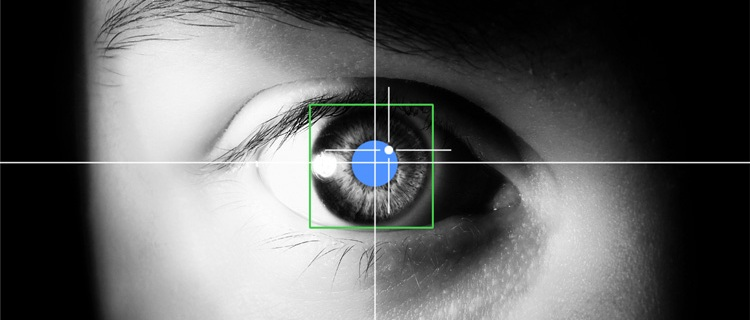
\includegraphics[width=0.60\textwidth]{images/eyetracker}
\end{figure}
\vspace{0.5 in}
{\centering \huge \color{accentcolor} \sc \textbf{\teamname \\ \productname} \par}
\vspace{0.5 in}
{\centering \large \sc \textbf{\authors} \par}
\newpage


%\vspace{1 in}
%\centerline{January 13th, 2012}
%\newpage

%%% Revision History
\begin{versionhistory}
  	\vhEntry{0.1}{10.07.2015}{JT|FN|ZA|KB|JS}{Project Charter Creation}
  	%\vhEntry{0.2}{10.05.2015}{AT|GH}{complete draft}
  	%\vhEntry{0.3}{10.12.2015}{AT|GH}{release candidate 1}
  	%\vhEntry{1.0}{10.20.2015}{AT|GH|CB}{official release}
  	%\vhEntry{1.1}{10.31.2015}{AL}{added customer change requests}
\end{versionhistory}
\newpage

%%% Table of contents
\tableofcontents
\newpage

%%% List of figures and tables (optional)
\listoffigures
%\listoftables
\newpage

%%% Agile project charter sections
\section{Vision}
Our vision is to create an eye tracking system to benefit the lives of those living with disabilities such as Amyotrophic lateral sclerosis(ALS). The system shall not only be very modern looking but it shall perform with great precision and it shall radically cut the cost compared to other present eye tracking systems. 
\section{Mission}
The mission of our project is to work as a team to design and develop an inexpensive eye tracking system which needs to:
\begin{itemize}
\item Look modern and sleek
\item Accurately track eye movement and must be bug free
\item Remain within or under the allocated budget 
\end{itemize}
How are we going to do this?
\begin{itemize}
\item Research the hardware modules: Cpyrus CX3, Odroid XU4, Infrared LEDs, MIPI Cameras and integrate them
\item Research and use open source eye tracking algorithms and integrate that into our system
\item Use C++ and openCV for processing information
\item Use LaTeX for the entire documentation
\end{itemize}

\section{Success Criteria}
After much deliberations, we came up with the following success criterias:
\begin {itemize}
	\item The design of the eye tracking device becomes visually appealing.
	\item The eye tracking device is comfortable to wear.
	\item The eye tracking is accurately calculated and visually represented without any bugs.
\end {itemize}
\newpage

%%% Remaining project charter sections
\section{Background}
Students of the CSE (Computer Science Engineering) department at the University of Texas at Arlington (UTA) are required to complete a Systems Design project also called \“Senior Design\” during the final year. Dr. Christopher McMurrough was the instructor for the class. During the beginning of the semester, each student was asked to submit an introductory essay that describes their interests, strengths, weaknesses, and any project ideas if they had any. Based on our essays, Dr. McMurrough formulated our team. We had five people on our team: Fernando Do Nascimento, Joseph Trinh, Krishna Bhattarai, Zachary Allen, and James Stone
A list of project topics was suggested for the entire class. After much deliberation and thoughts our team decided to go with the Eye Tracker project.

Eye Tracking is an emerging technology that tracks the eye movement of the user. It is particularly important when it comes to tracking eye movement of people that have ALS(Amyotrophic Lateral Sclerosis) which over the time paralyses all body parts except for the eye. Eye Tracking is also used by large supermarkets to collect data of where the customers are looking at most. Based on the data they collect from the ey tracker, they rearrange items on their shelves to increase profit. Current eye tracking systems that are commercially available are very expensive. They cost as much as 20,000 or more. 

In conclusion, our goal is to create an eye tracking system, that is not only affordable but also modern looking and one that performs with higher accuracy and speed. We are looking to improve the eye-tracking technology by making the product more affordable to a wider range of users without having to sacrifice the video processing quality and precision. Another goal of our project is to create a device that is comfortable to wear, since some of the users might use this product for an extensive period of time. Finally, our main goal is to improve the quality of life of people living with disabilities such as ALS.
\section{Related Work}
In the past decade eye-tracking systems have become very popular and in high demand since it has multiple applications. Some of the applications involve improving the living conditions of people living with Amyotrophic Lateral Sclerosis (ALS) or any other disease that affects the control movement of a person. Another application of the eye tracking involves marketing researching for companies selling products at convenience stores or supermarkets. Today, there are multiple eye-tracking systems being offered both open-source and commercially available products.

Most of the open-source eye-tracking systems available today involve using web cameras. Since, they are building a low cost system, the quality of the video being process has a lower quality compared to the camera that we will be using with the Cypress EZ-USB CX3. Another disadvantage is that some of these projects do not use a head-mounted system, so the program is less accurate tracking the eye gaze since it is performing the algorithm from a greater distance; this means that these types of eye-tracking systems are less accurate than head-mounted eye-tracking systems. There are also open-source systems that use head-mounted systems; in these systems they used two types of camera modules, web cameras and a digital camera. In the web camera system, the camera is directly connected to a computer. \cite{Kumar2006} While in the digital camera system, the camera is mounted in the enclosure that the camera came with along with making some modifications to the hardware. \cite{Unknown2015} The price of the open-source systems varies depending on the camera module to be used. 

The eye-tracking systems that are commercially available in today’s market are very expensive. The most affordable system that our research showed was \"\$99 USD\" \cite{TheEyeTribe2015} , other systems cost around \"\$22,000 USD.\" \cite{EyeTracking2011} The company of the most affordable system, The Eye Tribe, provides an API for the device so the buyer may use the product for multiple purposes. This device is not a head mounted device, so it is not practical to use, since it needs to be mounted on a device or surface in order to be used. The company, EYETRACKING, which created the \"\$22,000 USD\" \cite{EyeTracking2011} system, does not provide buyers with an API to operate the product for different uses. This company provides the buyers with a software suite in order to use their product. This company provides multiple types of eye-tracking systems both head-mounted and remote; some of the head-mounted system seems to be very bulky and uncomfortable to wear.
\section{System Overview}
This section should describe the overall structure of your software system. Think of it as the strategy for how you will build the system. An architectural "layer" is the top-level logical view, or an abstraction, of your design. Layers should be composed of related elements of similar capabilities, and should be highly independent of other layers, but should have very clearly defined interfaces and interactions with other layers. Each layer should be identified individually and should be unique as to its function and purpose within the system. This section should also contain the high-level block diagram of the layers, as shown in the example below, as well as detailed descriptions of the functions of each layer.

\begin{figure}[h!]
	\centering
 	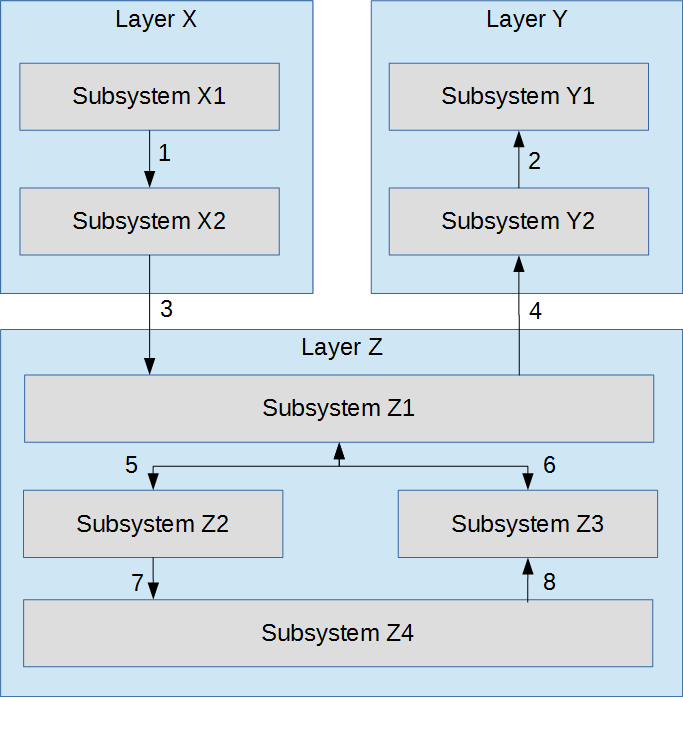
\includegraphics[width=0.60\textwidth]{images/data_flow}
 \caption{A simple architectural layer diagram}
\end{figure}

\subsection{Layer X Description}
Each layer should be described separately in detail. Descriptions should include the features, functions, critical interfaces and interactions of the layer. The description should clearly define the services that the layer provides. Also include any conventions that your team will use in describing the structure: naming conventions for layers, subsystems, modules, and data flows; interface specifications; how layers and subsystems are defined; etc. 

\subsection{Layer Y Description}
Each layer should be described separately in detail. Descriptions should include the features, functions, critical interfaces and interactions of the layer. The description should clearly define the services that the layer provides. Also include any conventions that your team will use in describing the structure: naming conventions for layers, subsystems, modules, and data flows; interface specifications; how layers and subsystems are defined; etc. 

\subsection{Layer Z Description}
Each layer should be described separately in detail. Descriptions should include the features, functions, critical interfaces and interactions of the layer. The description should clearly define the services that the layer provides. Also include any conventions that your team will use in describing the structure: naming conventions for layers, subsystems, modules, and data flows; interface specifications; how layers and subsystems are defined; etc. 
\section{Roles \& Responsibilities}

Project Organization: the key members of the project are:
\begin{itemize}

\item Scrum Master: Krishna Mani, computer science major

\item Project Owner: James Stone, computer science major 

\item Project Team Member: Fernando Do Nascimento, computer engineer, lead project documenter

\item Project Team Member: Zach Allen, computer science major

\item Project Team Member: Joseph Trinh, computer science major
\end{itemize}
\large Scrum Master Role/Responsibilities: removing any impediments that may obstruct a team’s progression towards a sprint goal.
\large Project Owner Role/Responsibilities: maintaining the product backlog, communicating between the project team members and the other stakeholders, managing the customer expectations and managing the budget.
\large Project Team Member Role/Responsibilities: identifying and assigning individual tasks, communicating the status of the project and issues being faced to the scrum master, and giving a demo of task completed during the project sprints to the project owner.
\section{Facilities \& Equipment}
The places we will be working will be the Senior Design lab and the FabLab.

The equipment available to us is the school provided computer and the 3D printer in the senior design lab.
\section{Cost Proposal}
\subsection{Preliminary Budget}
We have a budget of \$800 which was provided by the University. 
\section{Documentation \& Reporting}
\subsection{Project Charter}
The project charter is a key document when working on any type of project, since it states the objectives, scope, and schedule of the project. This document will be used to define what the Eye-Tracker project is, establish the structure of the project, show and explain the cost proposal for this project, and the roles and responsibilities of each member working on this project. Another task of this document is to display to the product owner and product managers, since it will compare this project to other related products and show the improvements of this project compared to the competitors.

\subsection{Product Backlog}
The product backlog will contain all the initial requirements of the Eye-Tracker project. As the project progresses, modifications to the requirements might develop. In the case, where changes to the requirements are necessary; then this document will be updated in order for the product owner, product manager, and/or future teams to be aware of the changes in the requirements and/or product. The changes to the requirements will be explained in the document, so anyone working on this project understands why the requirement has been modified. 

\subsection{Sprint Planning}
The scrum master, product owner, and every member of the scrum team are required to attend to every sprint-planning meeting. During the meeting, the team working on the project will agree to complete a set of tasks from the product backlog. Also, the team will be able to define the sprint backlog along with the estimated time for each task; depending on the task to be completed, some of the tasks might broken down to smaller tasks. Each sprint is between 2 to 4 weeks.

\subsubsection{Sprint Goal}
The sprint goal is a description of what the team working on the product is planning to complete during the sprint. This is done, so anyone outside of the project knows what the team is currently working on. During each sprint-planning meeting and as the project progresses, the sprint goal will change.

\subsubsection{Sprint Backlog}
The sprint backlog is a list of tasks that was defined by the scrum team during the sprint-planning meeting. Each tasks in the sprint backlog is chosen from the product backlog. Scrum team members are required to keep track of the amount of hours that they spent working on each task. While completing the tasks on the sprint backlog, new items might appear for future sprints.

\subsubsection{Task Breakdown}
In order to complete certain tasks of the sprint backlog, in some cases it is helpful to breakdown each task. This will help the scrum team member organize the completion of the task as well as precisely determine the estimated time that each task will take. This is similar to an algorithm known as divide and conquer, since both involve breaking down the problem until it becomes simple to solve.

\subsection{Sprint Burndown Charts}
During each sprint, the scrum team is required to have a sprint burndown chart. Inside this chart, the spreadsheet will contain the list of each task of the sprint along with the estimated time for the task, the amount of hours worked on each tasks during the 2 to 4 weeks period, the total number of hours that each member worked on each task, and the status of the sprint tasks. In order to keep track of the sprint goal progress, the sprint burndown chart will be uploaded to the Google Drive folder shared by the team working on the project, scrum master, and product owner. 

\begin{figure}[h!]
	\centering
	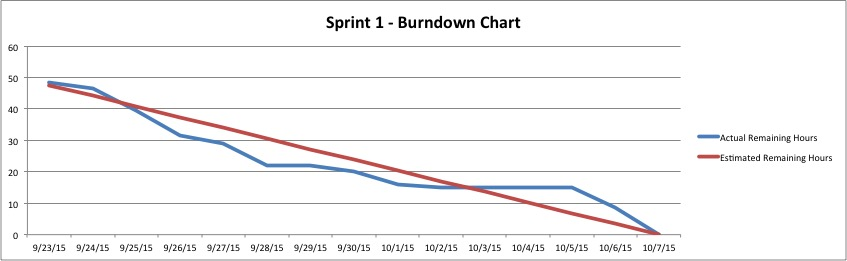
\includegraphics[width=0.90\textwidth]{images/chart}
	\caption{Sprint 1 Burndown Chart}
\end{figure}

\subsection{Sprint Retrospective}
During the sprint retrospective, the scrum master will discuss with each member of the team over the sprint session that just concluded. During this meeting, the team will also discuss what improvements can be made in order to make the future sprints more productive and successful. This meeting is very important for the project, since it may help improve the project throughout its completion. 

\subsection{Individual Status Report}
Throughout this project every member of the team is required to complete an individual status. In this report, each member will write down the task that the member has completed or is currently working on, along with the amount of hours spent on each tasks, and the future plans for the next sprint. Another item to mention in this report if while completing a task, another unexpected task appear.

\subsection{Engineering Notebooks}
Each member of the scrum team is required to obtain an engineering notebook. Inside this notebook, each member will write in detail any work performed that is related to this project. It is crucial for every member to be up to date with their entries in their engineering notebook, since it is a legal document and it is also checked periodically. 

\subsection{Closeout Materials}

\subsubsection{System Prototype}
During the life of this project, the scrum team will develop a functioning prototype of the Eye-Tracker. As the team makes progress on the project, modifications to the prototype will be performed. All the testing related to this project will be performed on this system prototype. Once the project is completed, the system prototype may be used to develop the final product. 

\subsubsection{Executive Summary}
The executive summary will give a summary of what the problem that the project is intended to solve. The purpose of this summary is for the readers to become familiar with the project without having to read all the documentation. Another purpose of this summary is to state the advantages and improvements compared to the competitors and the market that the product serves.

\subsubsection{Web Page}
The scrum team will create a static web page for advertising purpose of the product. The web page will contain pictures of the product along with the description of what the product performs, its functionality, and applications. The team will deliver the static web page in a flash drive.

\subsubsection{Demo Video}
The scrum team shall develop a video of the prototype performing its intended functions, the instructions necessary to operate the device, and an explanation of how the device performs its operations. The demo video might also be used for advertisement purpose. For better accessibility the video will be stored in a flash drive or a DVD.

\subsubsection{Source Code}
The scrum team will store the source code of the project in a Github repository for accessibility purpose while developing the product. Once the project is completed, the team will store the all the source code related to the project on a flash drive. At the moment, the product will involve programming in C++ and use the openCV library module.

\subsubsection{Source Code Documentation}
The scrum team will keep very detailed documentation in all source code related to this project. The purpose of the source code documentation is to explain how each function of the program works, so current team members or future teams that make modifications to the product do not have to expend unnecessary time attempting to understand how each function works.

\subsubsection{Hardware Schematics}
This project involves interfacing multiple hardware devices (Odroid XU4, Cypress EZ-USB CX3, and a camera module), multiple electronic components (IR LED, resistors, etc.), and a power. A schematic diagram of the product is a vital documentation that this team will provide.The schematic diagram will be stored in a flash drive as a JPEG format and in a format that the schematic diagram may be opened and altered when making modifications on future improvements.

\subsubsection{User Manual}
This scrum team will provide a user manual that will explain if any software is necessary to be installed in order to operate the product and any instructions necessary to properly operate the device. It will contain safety precautions and show pictures of how to operate the system. The documentation will be provided as PDF format and it will be stored in a flash memory.
\newpage

%%% References
\bibliographystyle{plain}
\bibliographystyle{reference/IEEEtran_custom}
\bibliography{reference/refs}{}

%% The following is another way of doing references manually!
%\begin{thebibliography}{1}
%\bibitem{EyeTracking2011} EyeTracking {http://www.eyetracking.com/Hardware/FOVIO-Eye-Tracker} 1991
%\bibitem{Kumar2006} Kumar, Manu {Reducing the Cost of Eye Tracking Systems} 2006

%\end{thebibliography}


\end{document}